\documentclass[10pt,a4paper]{labreport}
\usepackage{csquotes}
\usepackage{titlesec}
\usepackage{ragged2e}
\usepackage{siunitx}
\usepackage{setspace}
\usepackage{longtable}
\usepackage{rotating}
\usepackage{xurl}
\usepackage{physics}
\usepackage{caption}
\usepackage{wrapfig}
\usepackage{tabularray}
\usepackage{fancyhdr}
\usepackage{subcaption}
\usepackage{lscape}
\usepackage{tensor}
\usepackage{multirow}
\usepackage{chemformula}
\usepackage[gen]{eurosym}
\usepackage{float}
\usepackage{bm}
\usepackage{lipsum}
\usepackage{parskip}
\usepackage{booktabs}
\usepackage{enumerate}
\usepackage[justification=justified]{caption}
\usepackage[nottoc]{tocbibind}
\usepackage{color}

\usepackage{listings}
\definecolor{codegreen}{rgb}{0,0.6,0}
\definecolor{codegray}{rgb}{0.5,0.5,0.5}
\definecolor{codepurple}{rgb}{0.58,0,0.82}
\definecolor{backcolour}{rgb}{0.95,0.95,0.92}
\lstdefinestyle{mystyle}{
    backgroundcolor=\color{backcolour},   
    commentstyle=\color{codegreen},
    keywordstyle=\color{codepurple},
    numberstyle=\tiny\color{codegray},
   % stringstyle=\color{grey},
    basicstyle=\ttfamily\footnotesize,
    breakatwhitespace=false,         
    breaklines=true,                 
    captionpos=b,                    
    keepspaces=true,                 
    numbers=left,                    
    numbersep=5pt,                  
    showspaces=false,                
    showstringspaces=false,
    showtabs=false,                  
    tabsize=5
}
\lstset{style=mystyle}
\usepackage{hyperref}
 \usepackage[
backend=biber,
style=chem-acs,articletitle=true,doi=true]{biblatex}
\addbibresource{references.bib}





\title{Nanoscale Material Modelling
\\
\normalsize{Week 4}} % Main title and sub title. 

\author{Ilija A. Gjerapić, S4437586; \href{mailto:i.a.gjerapic@student.rug.nl}{i.a.gjerapic@student.rug.nl}; \href{https://github.com/igjerapic/nmm-week4/}{@github} } % Name, student number, email

\supervisors{prof. dr. A. Giuntoli, prof. dr. J. Slawinska}

\begin{document}


\maketitle
\tableofcontents


  

\thispagestyle{firststyle}
\newpage
\section{Assignment 1: The Icebreaker}
The TIP3P and TIP4P models of water were used to model the melting of ice I$_\text{H}$ by increasing the simulation temperature from 0K to 1000K. 
The main differences between these two models is the location of the charges. 
TIP3P has each charge localized at the center of each atom, while the TIP4P model localizes the charge of the Oxygen closer to the two hydrogen atoms in a forth massless particle. 
Table \ref{tab:ass1_lammps-bonds} shows the difference in efficiency between the two models.

\begin{table}[h]
    \caption{A comparison between the efficiency of the two water models. The introduction of the fourth, massless particle in the TIP4P water model results in an efficiency drop of around 55\%, when considering timesteps/s. }
    \label{tab:ass1_lammps-bonds}
    \centering
    \begin{tabular}{ccc}
      \hline
    \textbf{Water Model}      & \textbf{hours/ns}     & \textbf{timesteps/s}   \\
    \hline
    TIP3P & 0.225 & 1233.335 \\
    TIP4P & 1.363      & 679.128  \\ \hline
    \end{tabular}
\end{table}

The radial distribution function  (RDF) at increasing temperatures for the \texttt{TIP3P} model and \texttt{TIP4P} are shown in Figure \ref{fig:ass1_rdf}(a) and \ref{fig:ass1_rdf}(b), respectively. It is clear that at higher temperatures, the strucure for both models becomes more liquid like as the sharp peaks disipate. This is clearer when visualizing the initial and final structures of the two models as shown in the insets of Figure \ref{fig:ass1_OH-bonds}.

However, peaks at 1.0 {\AA} and 1.5 {\AA} are persistant no matter the temperature. This is as these peaks relate to single water molecules: the peak at 1.0 {\AA} corresponds to the distance between the oxygen and hydrogen atoms, while the peak at 1.5 {\AA} is due to the fixed distance of the two hydrogen atoms.
  
\begin{figure}[h]
  \centering 
  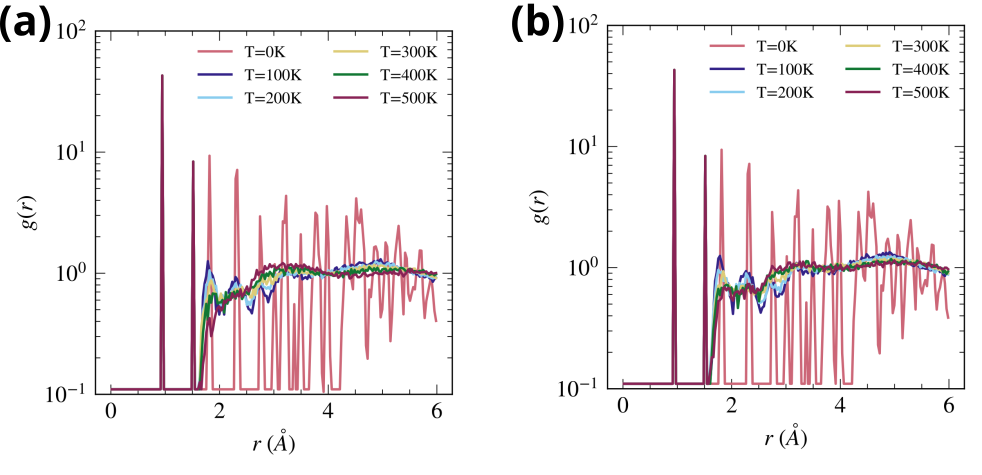
\includegraphics[width = 0.7\textwidth]{figs/ass1_rdfs.png}
  \caption{\textbf{(a)} The radial distribution function of \textbf{(a)} the TIP3P water model and \textbf{(b)} the TIP4P water model. The first peak at approximately 1 {\AA} corresponds to the distance between the oxygen and hydrogen of the same water molecule, while the second peak at approximately 1.5 {\AA} is due to the distance between the two hydrogens within the same water molecule.}
  \label{fig:ass1_rdf}
\end{figure}

  The point at which the ice melts can be estimated by considering the temperature at which the number of O-H intermolecular bonds reaches a new equilibrium. 
  Figure \ref{fig:ass1_OH-bonds} shows that the melting temperature of the \texttt{TIP3P} is about 500 K while the \texttt{TIP4P} reaches equilibrium around 600 K. 
  Both results differ significantly from the well-known value of around 300 K and reported simulation values of 146 K for TIP3P and 232 K for TIP4P \cite{vegaMeltingTemperatureMost2005} at pressures of 1 bar. 
  
  A possible reason for the large discrepancy between the simulated values of the melting temperature and the literature values in reference \cite{vegaMeltingTemperatureMost2005} is different simulated environments. 
  Mainly, our simulations were integrated using a \texttt{nvt}, keeping the volume of the simulation cell constant, while allowing for differences in pressures. This is fundamentally different from every day experience and the provided simulations in which the pressure is maintained.   

\begin{figure}[h]
  \centering 
  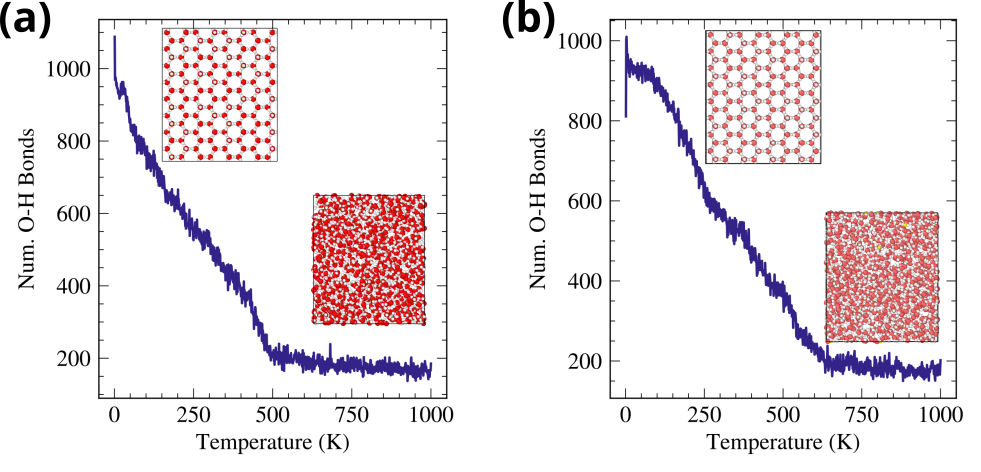
\includegraphics[width = 0.7\textwidth]{figs/ass1_OH-bonds.png}
  \caption{\textbf{(a)} The number of OH bonds created using \texttt{Ovito} as a function of the simulation temperature for \textbf{(a)} the TIP3P water model and \textbf{(b)} the TIP4P water model. The insets show visualizations of the initial (left) and final (right)  configuration of both simulations. The plateau of OH bonds indicates the melting of the ice showing a melting temperature of around 500 K for TIP3P model and 600 K for the TIP4P model.}
  \label{fig:ass1_OH-bonds}
\end{figure}




\newpage\newpage
\section{Assignment 2: Out of Flatland}
\subsection{Model Info}
\begin{itemize}
  \item \textit{What force field is used?}
  
  The \texttt{Airebo-m.C} force field for carbon is used. It is a reactive force field, and more specifically an Adaptive Intermolecular Reactive Empirical Bond Order Potential.

  \item \textit{Number of covalent bonds in the graphene sheet?} 
  
  The graphene sheet contains 3840 carbon atoms, which makes sense as the graphene sheet was defined to contain 40x24 rectangular unit lattices of carbon, each containing 4 carbon atoms.

  The total number of covalent bonds in the graphene sheet is technically zero as no bonds were defined in LAMMPS, but rather interatomic interactions.
  
  \item \textit{Key command line used to deform the graphene sheet?}
  
  The graphene sheet is deformed using the \texttt{fix indent} LAMMPS command as shown in listing \ref{lst:ass2_deform_command}. The command forms a sphere centered at the origin whose radius decreases at a fixed rate and indents all atoms within the sphere. To   
  \begin{lstlisting}[ 
    caption={The key commands used for deforming the carbon sheet.},
    label=lst:ass2_deform_command,
    ]
variable r0 equal (ylo^2+xlo^2+zlo^2)^0.5
variable r0fix equal ceil(${r0})                                     
variable rate equal 1.25      #A/ps
variable deltat equal "dt"
variable radius equal "v_r0fix-step*dt*v_rate"
fix constrain all indent 1 sphere 0 0 0 v_radius side in units box

# following command was used for tube/cylinder formation
fix constrain all indent 2 cylinder x -${yside} 0 v_radius side in units box
\end{lstlisting}
\end{itemize}
\newpage
\subsection{Running simulation}
Figure \ref{fig:ass2_configs_sphere} and \ref{fig:ass2_configs_tube} shows the midpoint and final configuration with the atoms colored by their potential energy for the spherical and cylindrical deformation, respectively. 
\begin{figure}[h]
  \centering 
  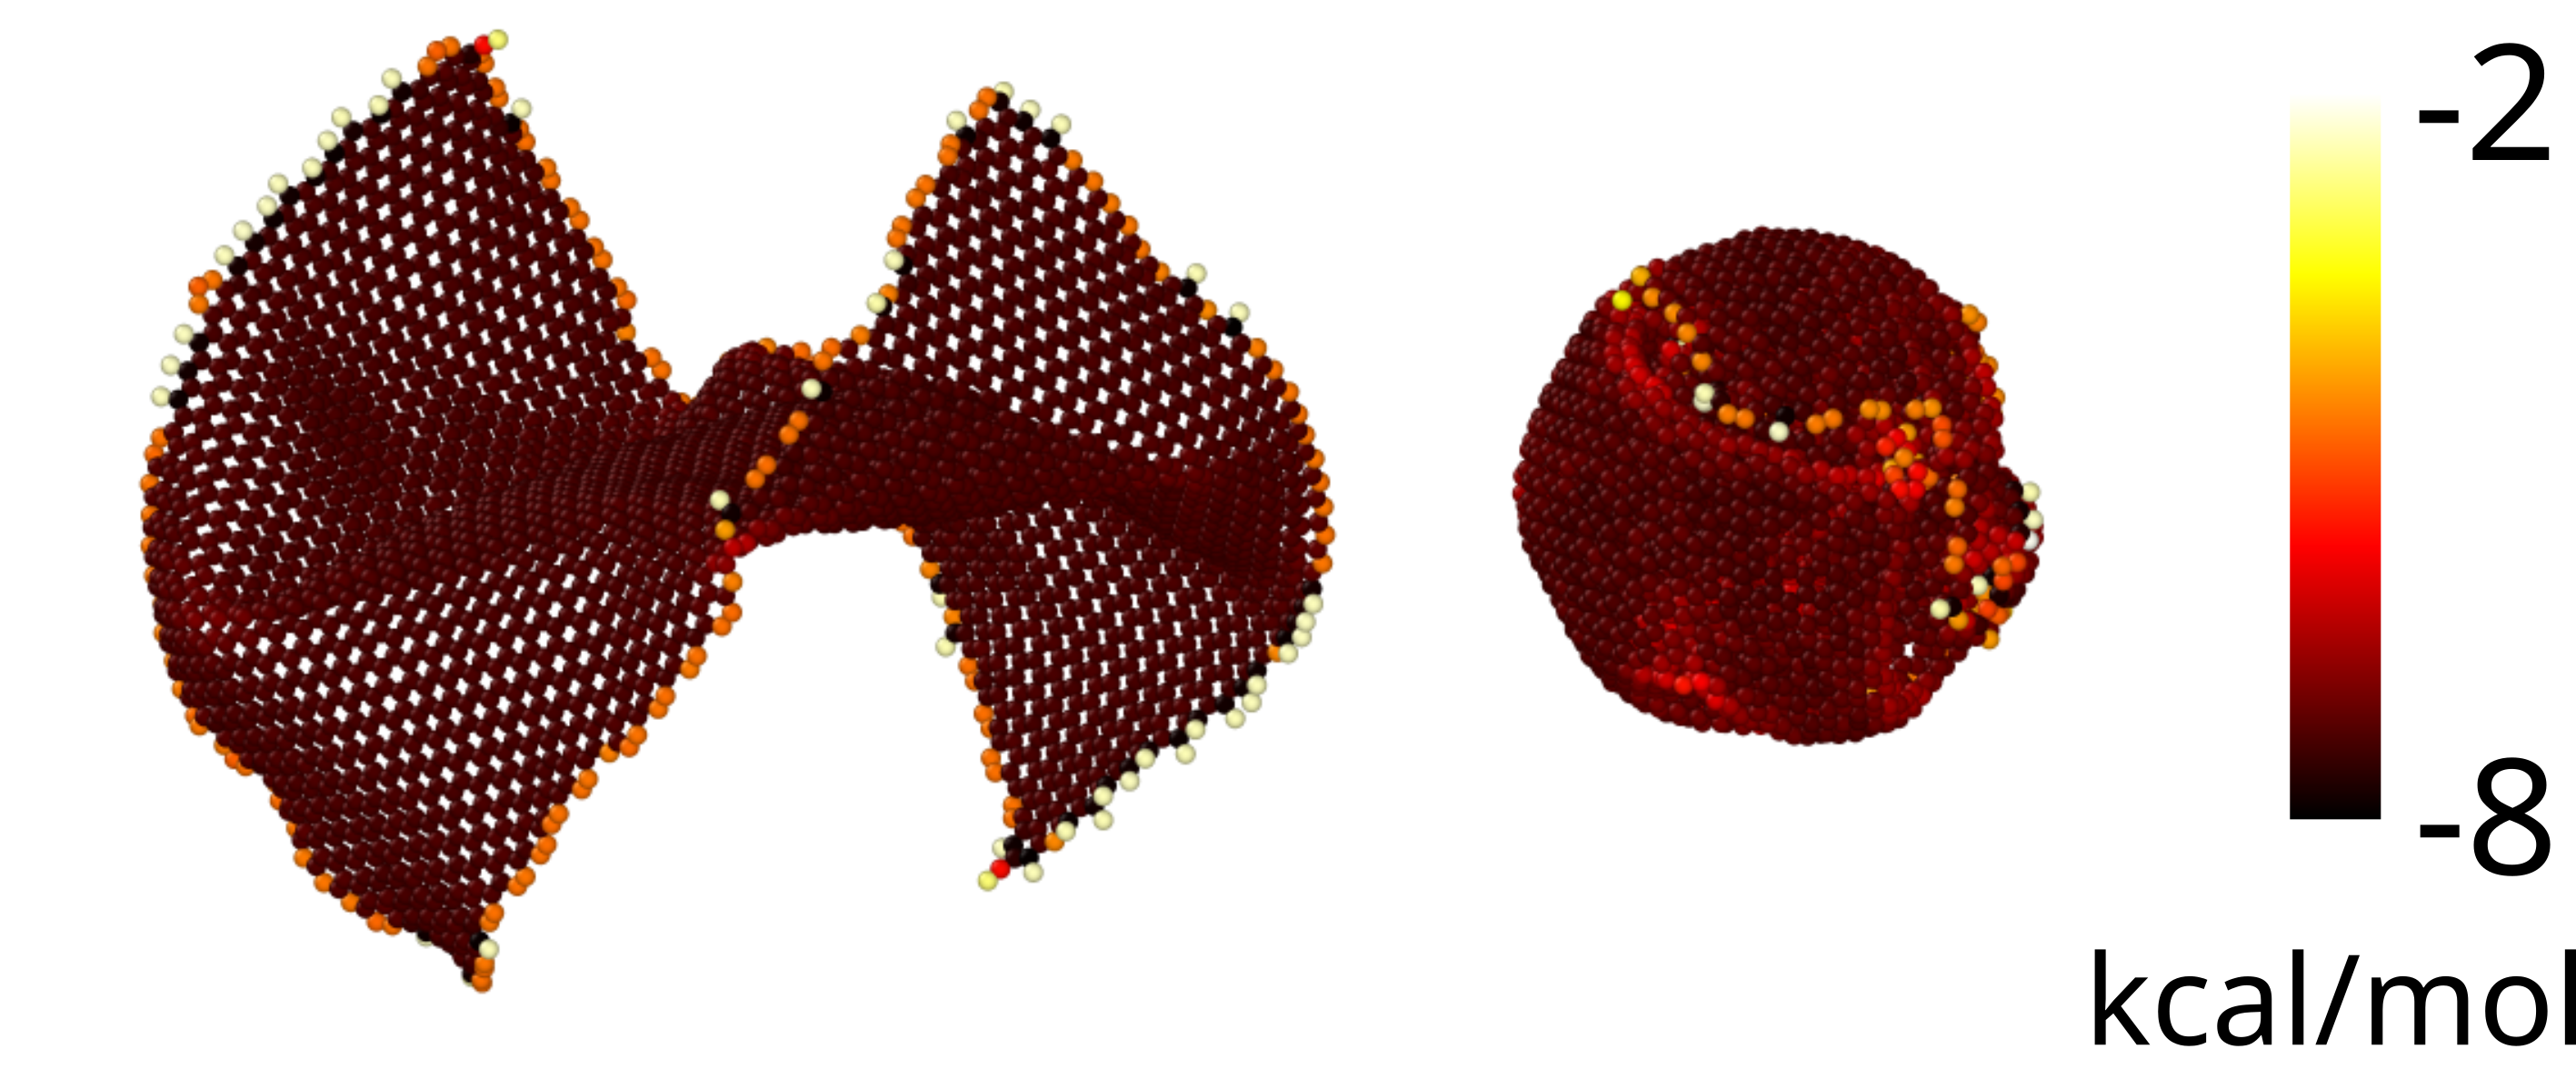
\includegraphics[width = 0.8\textwidth]{figs/ass2_poteng_sphere.png}
  \caption{\texttt{Ovito} snapshots of the spherical deformation of the graphene sheet at the midpoint (left) and end (right) of the simulation. The coloring corresponds to the potential energy of each atom. Atoms at the edge have the highest potential energy. }
  \label{fig:ass2_configs_sphere}
\end{figure}

\begin{figure}[h]
  \centering 
  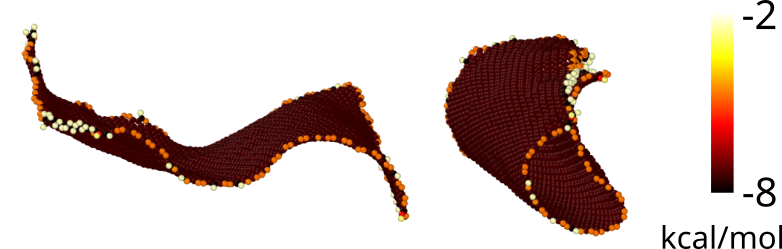
\includegraphics[width = 0.8\textwidth]{figs/ass2_poteng_tube.png}
  \caption{\texttt{Ovito} snapshots of the tube deformation of the graphene sheet at the midpoint (left) and end (right) of the simulations. The coloring corresponds to the potential energy of each atom. Atoms at the edge have the highest potential energy. }
  \label{fig:ass2_configs_tube}
\end{figure}
It is noticed that during the deformation, the atoms at the edge, in contact with the indent have the highest potential energy. Furthermore, it seems as if the spherical deformation leads to a more stressed system with a higher potential energy. This is confirmed when comparing the total potential energy further touched upon in Figures \ref{fig:ass2_rgs_sphere}(a) and \ref{fig:ass2_rgs_tube}(a). Furthermore, the radius of gyration of the sphere is much smaller than that of the carbon nanotube (Figures \ref{fig:ass2_rgs_sphere}(b) and \ref{fig:ass2_rgs_tube}(b) ). 



\begin{figure}[h]
  \centering 
  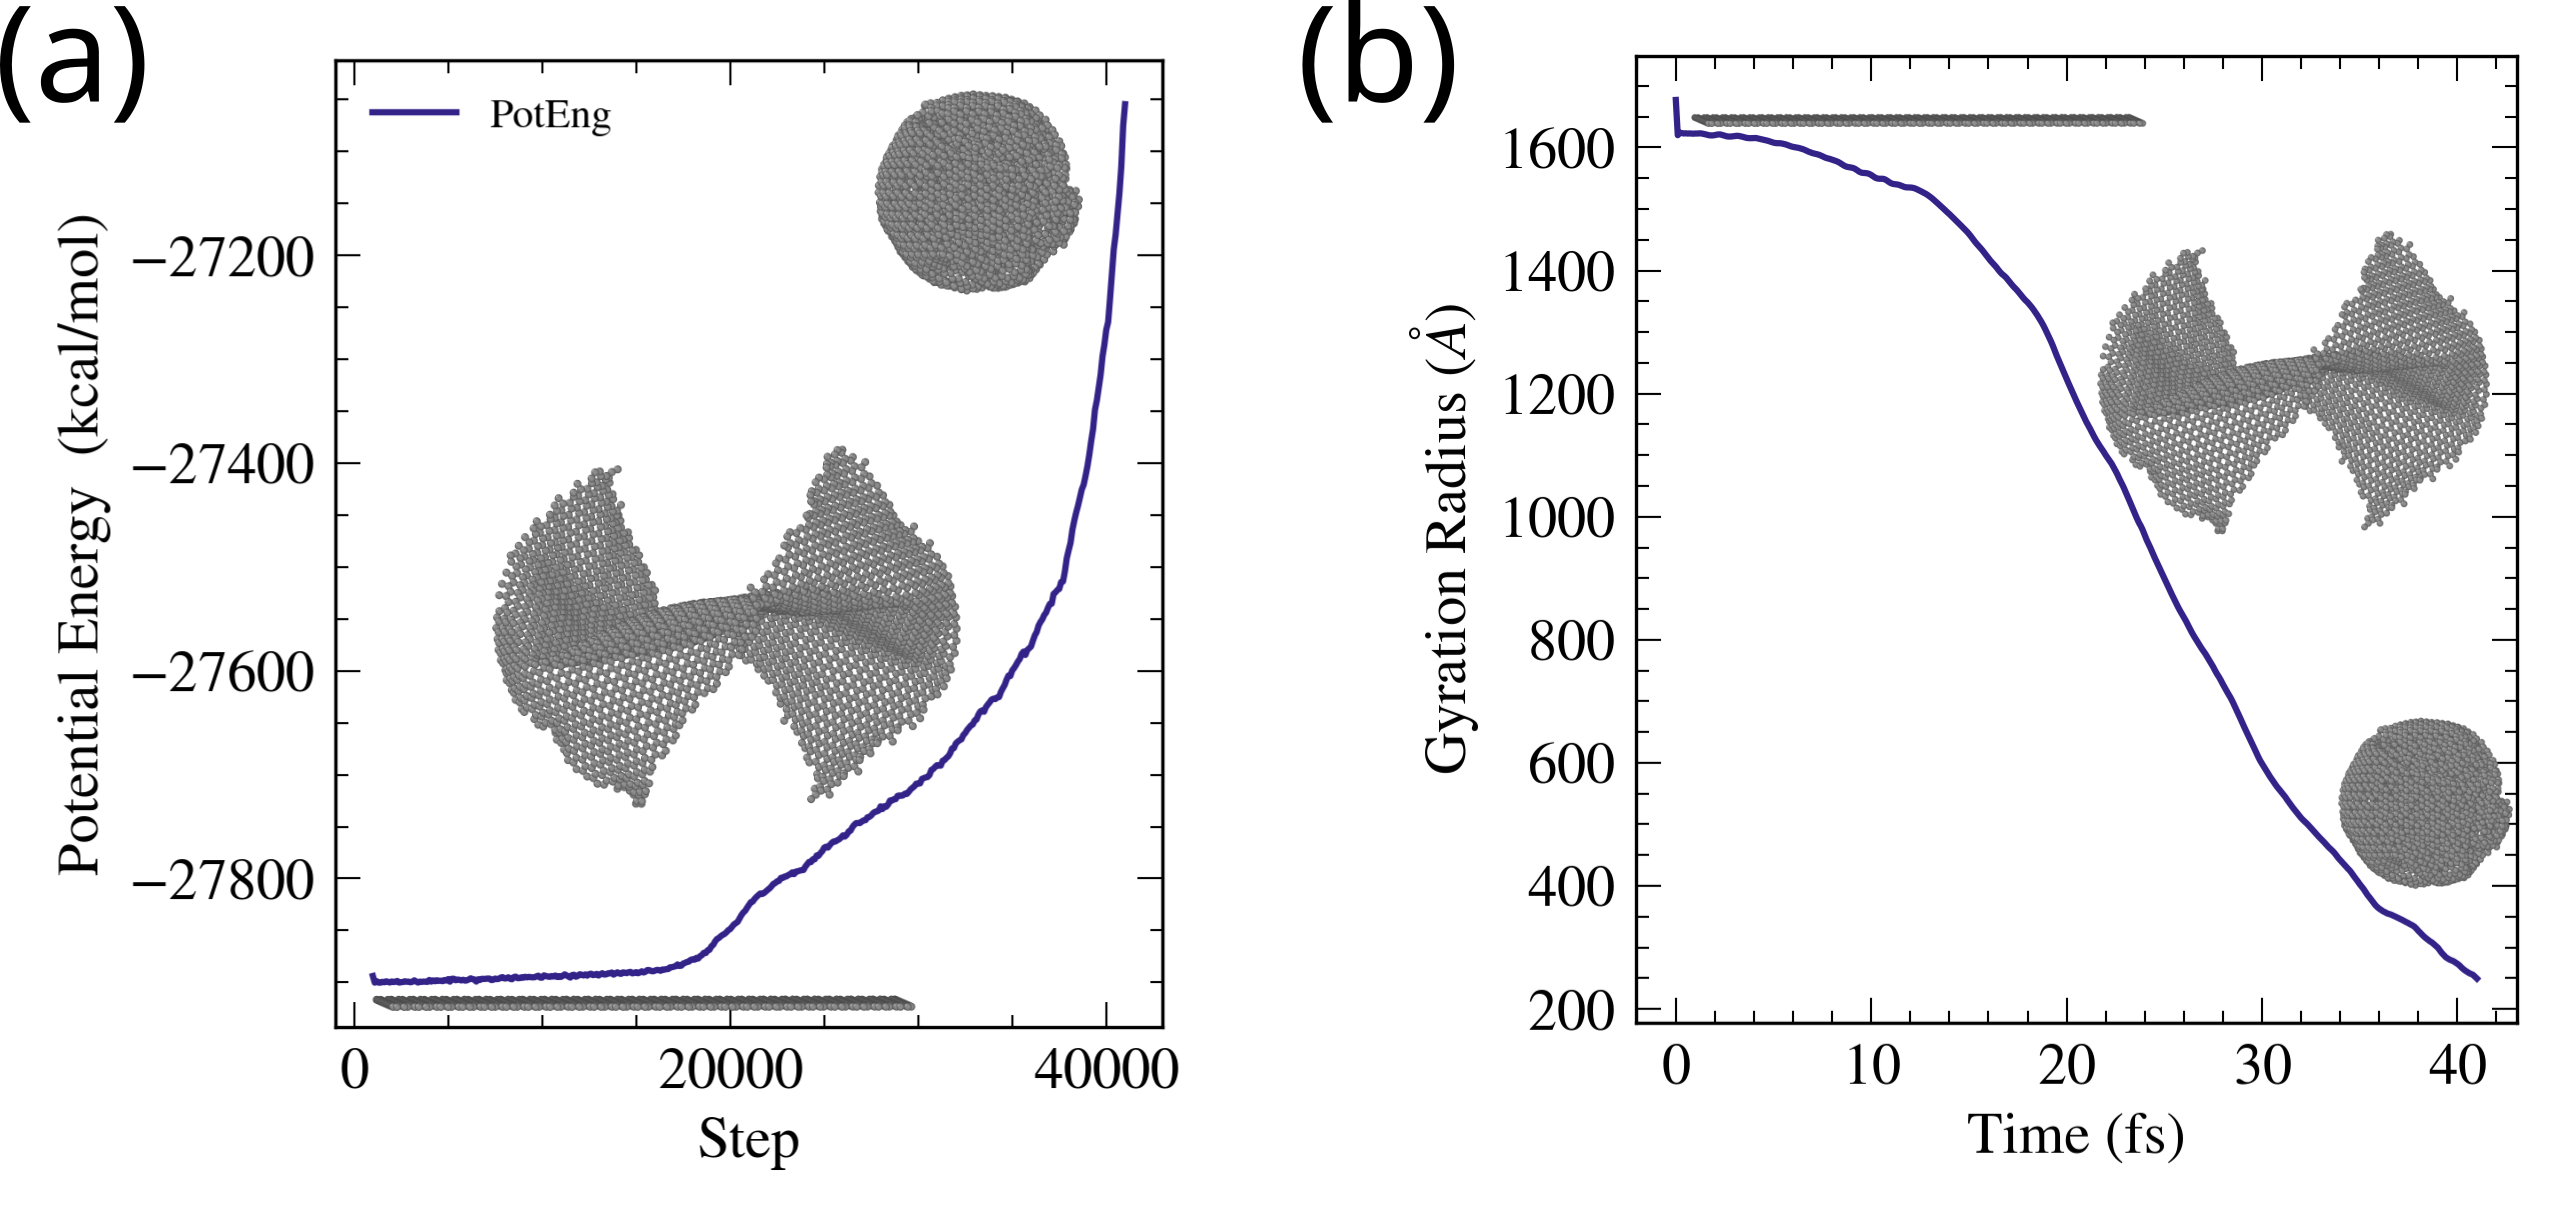
\includegraphics[width = 0.8\textwidth]{figs/ass2_rg_sphere.png}
  \caption{The (a) potential energy and (b) radius of gyration of the entire system throughout spherical deformation. The insets show (from left to right) the initial configuration, the midpoint configuration and the final configuration. }
  \label{fig:ass2_rgs_sphere}
\end{figure}

\begin{figure}[h]
  \centering 
  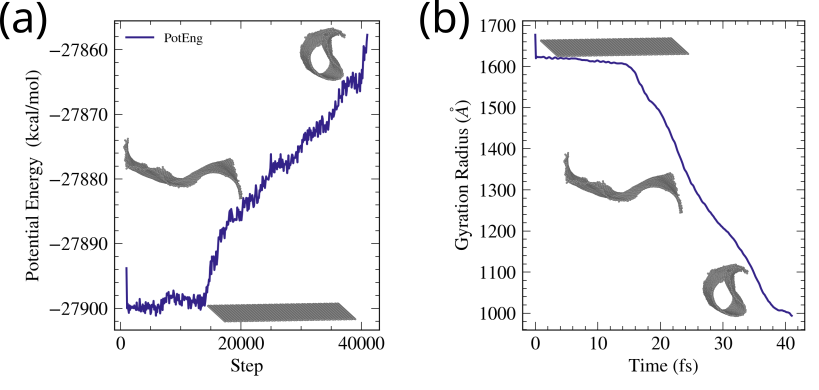
\includegraphics[width = 0.8\textwidth]{figs/ass2_rg_tube.png}
  \caption{The (a) potential energy and (b) radius of gyration of the system throughout the cylindrical deformation. The insets show the initial configuration, the midpoint configuration and the final configuration. }
  \label{fig:ass2_rgs_tube}
\end{figure}

\newpage
\subsection{Uniaxial deformation}
Uniaxial deformation was achieved using the \texttt{fix deform} command with an engineering strain rate of 0.01 while the positions of the carbon atoms were remapped. Listing \ref{lst:ass2_strain_command} shows the implementation of this.  
  \begin{lstlisting}[ 
    caption={The key commands used for deforming the carbon sheet.},
    label=lst:ass2_strain_command,
    ]
# Creating uniaxial extention to graphene sheet
variable finalstrain equal 1.0
variable rate equal 0.01
variable deltat equal "dt"
variable numberofsteps equal round(${finalstrain}/(${rate}*${deltat}))

print "Deforming box in x direction from L(t) = L0 (1 + 0.01 * dt) for ${numberofsteps} steps"
fix extension all deform 1 x erate ${rate} remap x units box  # remapped set to positions not velocities
\end{lstlisting}

After a strain of 42.8\%, the graphene sheet fails at multiple points as shown in Figure \ref{ass2_failure}. This is likely due to the fact that our simulated sheet is without impurities and thus initially without localized stress that can propagate. 
 
\begin{figure}[h]
  \centering 
  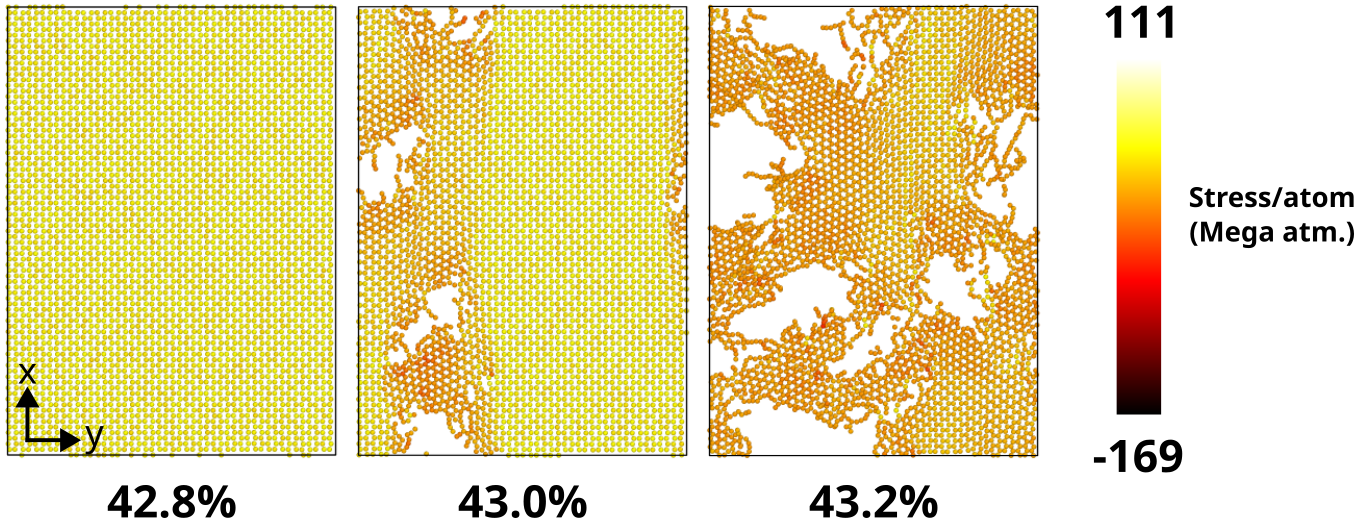
\includegraphics[width = 0.95\textwidth]{figs/ass2_strain.png}
  \caption{The progression of the carbon sheet failure with increasing system strain. The carbon atoms are colored by the stress/atom. The snapshots are taken within a timeframe of 0.6 fs. There is no specific point at which the failure propagates from.  }
  \label{fig:ass2_failure}
\end{figure}

\newpage\newpage
\section{Assignment 3: Go with the Flow}
\subsection{Model info}
\begin{itemize}
  \item \textit{What force fields are used to simulate water and graphene?}
  
  The force fields used to simulate water and graphene are separated into bonded and non-bonded interactions. 
  The bonded interactions include harmonic bonds, harmonic angles, opls dihedrals and harmonic impropers. The coefficients for these bonded interactions were set according to the GROMOS53A6 force field for carbon and the TIP4P force field for the water molecules. 

  The non-bonded interactions were set using the \texttt{pair\_style  lj/cut/tip4p/long} command from LAMMPS. This sets the interaction between oxygen and hydrogen atoms to be that of the TIP4P force field, while other non-bonded interactions are a LJ potential. 
 
  \begin{lstlisting}[ 
    caption={The command for the non-bonded interactions for water and carbon system. The first two numbers correspond to the atom ids to which the TIP4P force field applies. The next two numbers are the id for the O-H bond and the H-O-H bond angle, respectively. The second to last number is the distance of the massless charge site from the center of the oxygen. The final number is Coulombic interaction and global LJ cutoff. },
    label=lst:ass3_pair_style,
    ]
pair_sytle lj/cut/tip4p/long 1 2 1 1 0.105 10
\end{lstlisting}

  \item \textit{What is the value of the interaction energy epsilon between oxygen and carbon atoms?}
  \item 
  The interaction energy $\epsilon$ between the oxygen and carbon atoms is not directly specified, but determined by the arithmetic mixing rules:
  \begin{equation}
    \epsilon_{i\neq j} =  \sqrt{\epsilon_i\epsilon_j}
  \end{equation}
  Which gives $\epsilon_\text{O-C} = \sqrt{0.18481 \cdot 0.0663} = 0.11069$. 
  \item \textit{Which command enforces the flow of water in the channel?}
  \item 
  The \texttt{fix addforce} command enforces the flow of water in channel through the below implementation.
    \begin{lstlisting}[ 
    caption={The command enforcing the flow of water in the channel. The flow is thus in the x-direction.},
    label=lst:ass3_water_force,
    ]
variable    frc equal 2e-4
group       water type 1 2 # 1 is O, 2 is H
fix         kick water addforce ${frc} 0.0 0.0
\end{lstlisting}
  
\end{itemize}
\newpage 
\subsection{Running simulation}
\begin{itemize}
  \item \textit{Calculate the layer-by-layer distribution of water molecules' mass and velocity profiles along the z-axis. How does the velocity profile compare to what is expected for macroscopic laminar flow? What is the reason for the discrepancy?}
  
  Both the velocity and mass profiles seem to be quite homogeneous throughout the channel, if we ignore the noise. This is quite different from the parabolic profile of laminar flow. 
  
  The difference is likely due to the non-bonded interaction of the Oxygen and Carbon being set by the mixing rules, which can lead to results quite different than interactions optimized against the wetting angle of water on graphene \cite{liaoWaterGrapheneNonbondedInteraction2022}.
  
  Furthermore, to achieve a laminar flow, there must be a no-slip boundary, which is not observed in our simulations. 
  \begin{figure}[h!]
  \centering 
  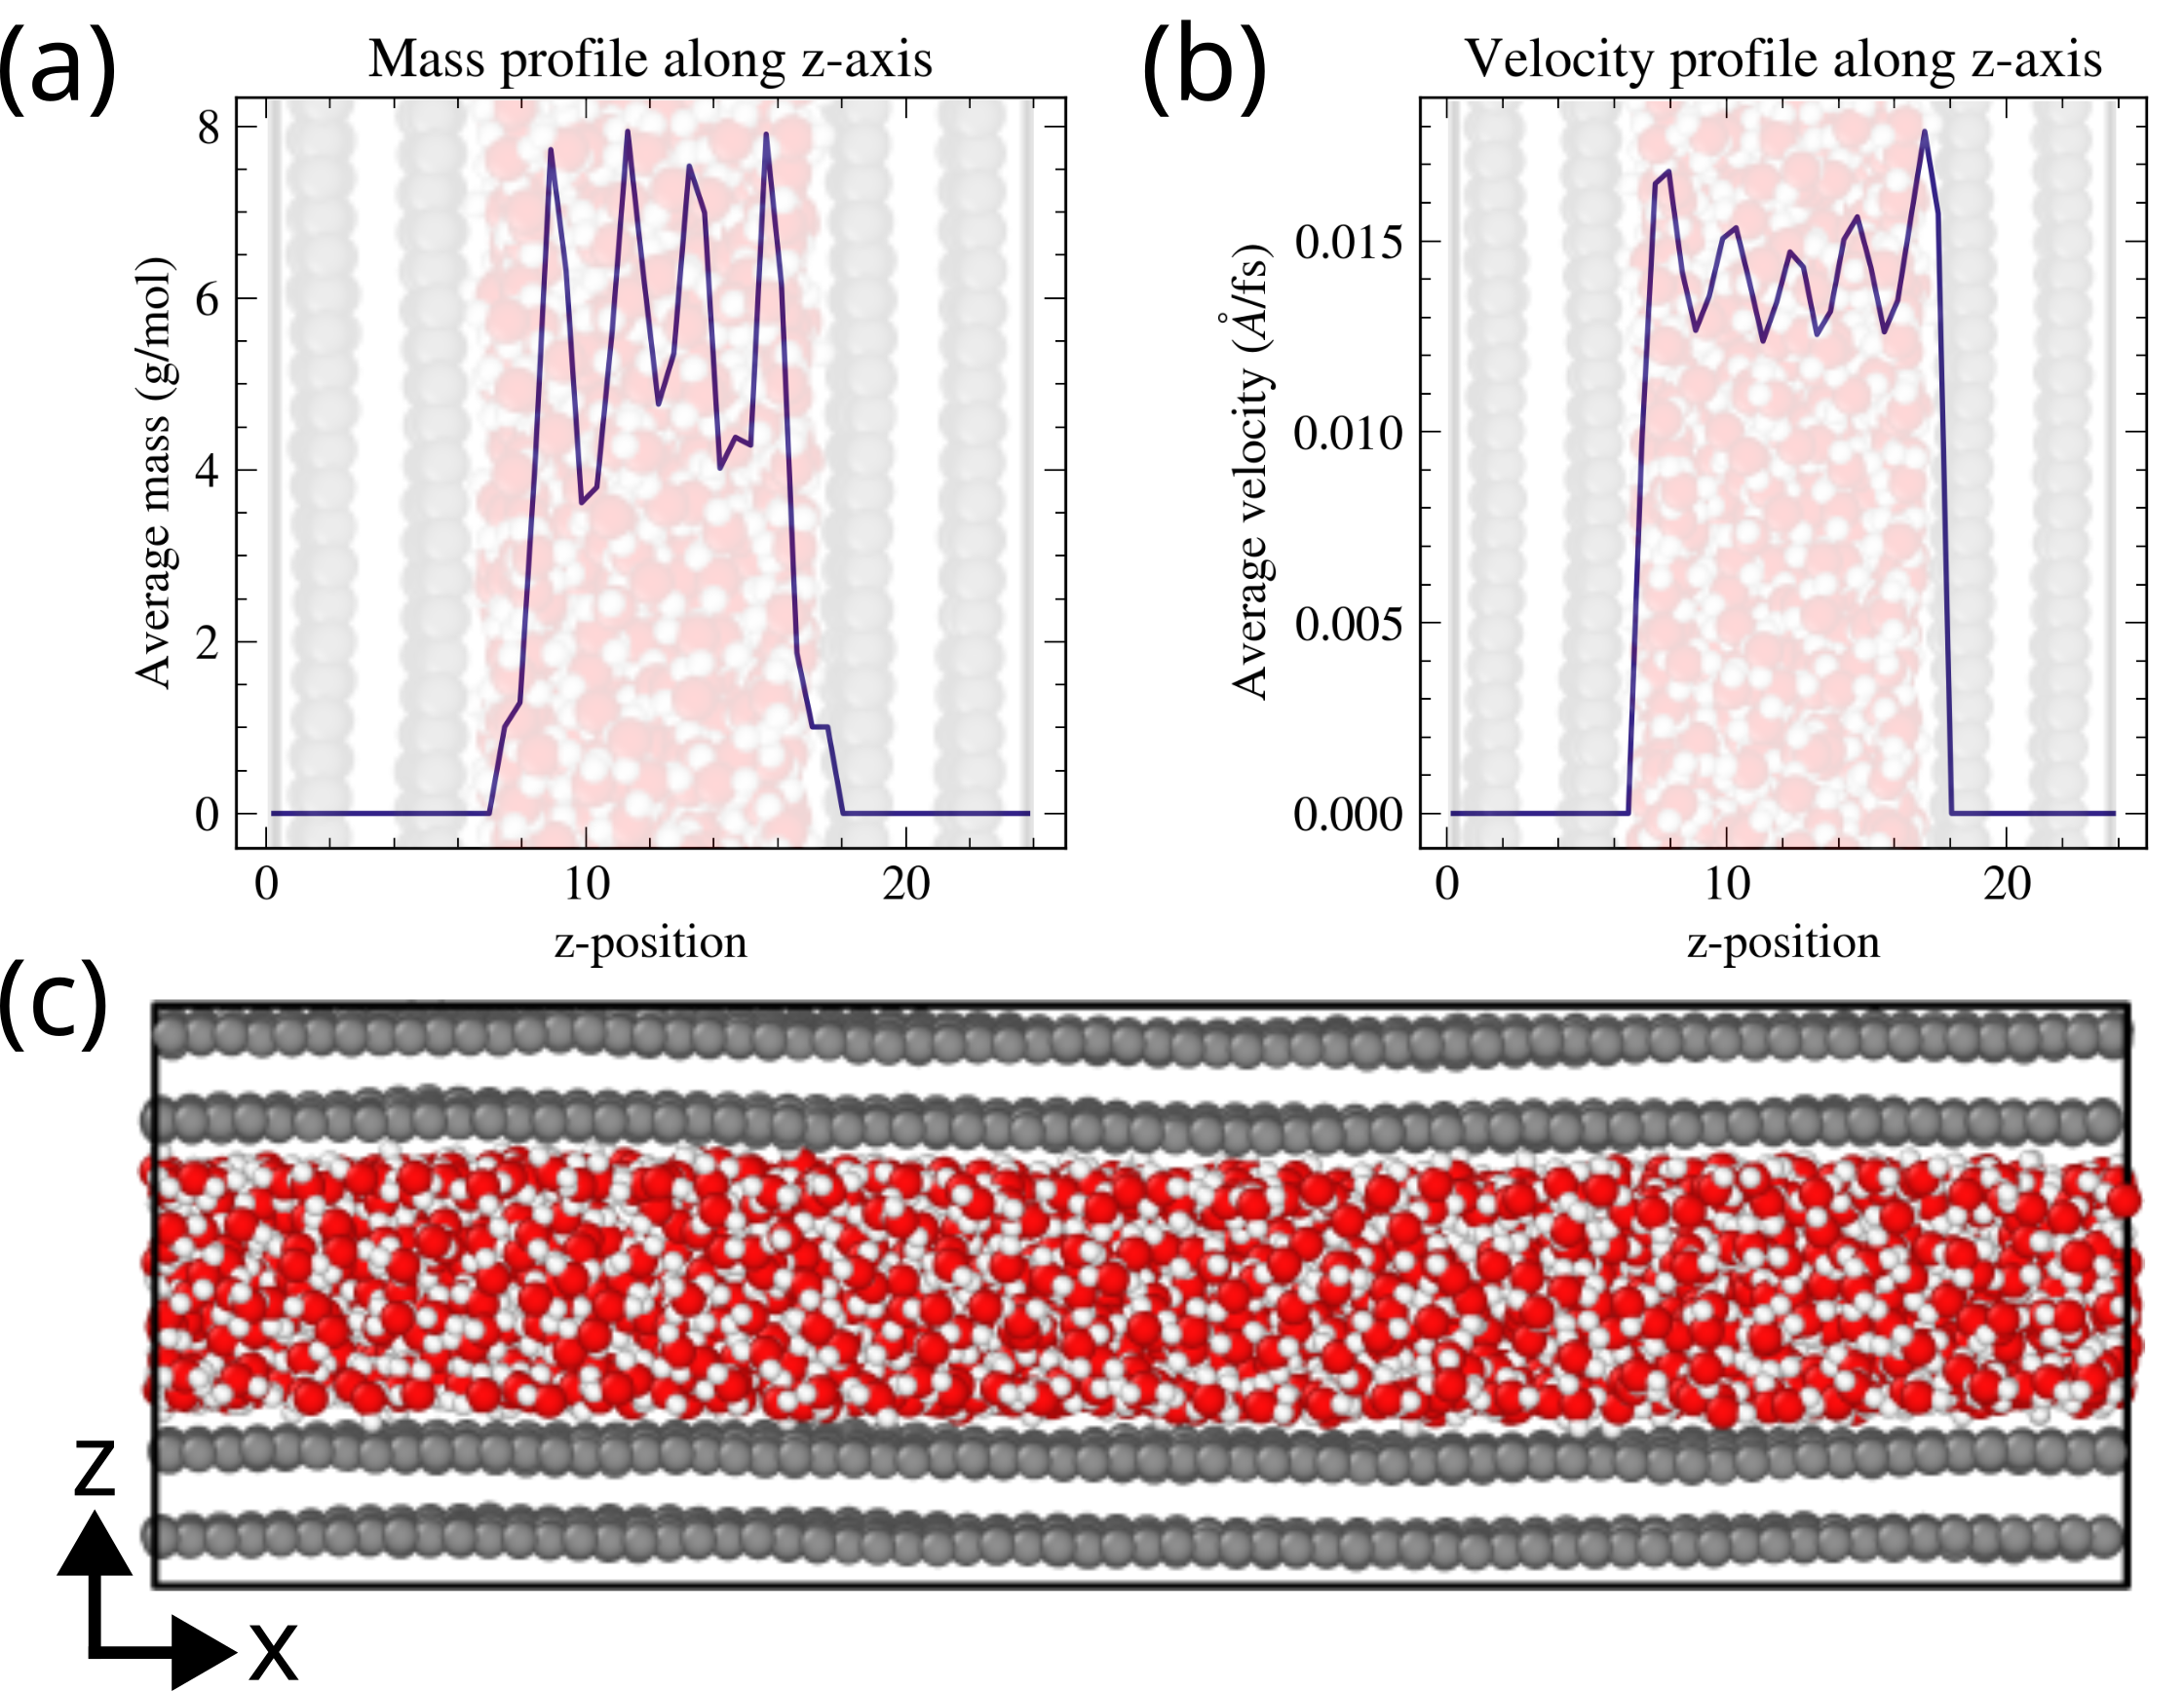
\includegraphics[width = 0.8\textwidth]{figs/ass3_profiles.png}
  \caption{The results from running the simulations. (a) shows the layer-by-layer mass distribution while (b) shows the average velocity profile. (c) is an \texttt{Ovito} visualization of the channel.  }
  \label{fig:ass2_failure}
\end{figure}

\item \textit{To obtain Poiseuille flow, a bound layer of fluid is expected to be present near the tube walls. Where does this effect come from, and how would you address this in your simulation?}

The bound layer present near the tube walls is due to the attractive interaction between the tube walls which cause the water atoms to stick on the wall. When the atoms diffuse away from the wall, their velocity increases due to momentum transfer between the diffusing water molecules and the flowing molecules. This is what leads to a parabolic velocity profile with a maximum at the center of the channel. 

To address the no-slip condition in the simulation, we can introduce regions within a certain distance from the carbon atoms forming the channel wall. Within this region, we can potentially enforce water molecules to stay stationary. 

To model the diffusion, the water molecules in the previously defined no-slip region could have a probability of being let free to move in line with a Boltzmann distribution. 
  
\end{itemize}



\newpage
\printbibliography

\appendix
\section{Code for Velocity Profile}
\begin{lstlisting}[language=python,
    caption={Main code snippet for determining the velocity profile in the channel.},
    label=lst:ass3_water_force,
    ]
    # Set up binning along z-axis, values taken to match mass profile 
    bin_count = 50
    z_min = 0.0
    z_max = u.dimensions[2]
    z_edges = np.linspace(z_min, z_max, bin_count + 1)
    z_centers = 0.5 * (z_edges[:-1] + z_edges[1:])

    # initializing arrays
    accumulated_velocity = np.zeros(bin_count)
    n_atoms = np.zeros(bin_count)
    average_vel = np.zeros(bin_count)

    # Compute speeds for atoms in water molecules for each trajectory 
    for i, traj in enumerate(u.trajectory):
        waters = u.select_atoms("type 1 or type 2")
        positions = np.array(waters.positions.copy())
        velocities = np.array(waters.velocities.copy())
    
        # compute n_atoms and individual attom speed for each bin 
        for j in range(1, len(z_edges)):
            mask = (positions[:,-1] >= z_edges[j - 1]) & (positions[:,-1] <= z_edges[j])
            n_atoms[j - 1] += len(positions[mask])
            for velocity in velocities[mask]:
                accumulated_velocity[j - 1] += np.linalg.norm(velocity)   

    # Average accumulated speeds by total number of atoms 
    for idx in np.nonzero(n_atoms):
        average_vel[idx] = accumulated_velocity[idx] / n_atoms[idx]
    plt.plot(z_centers, average_vel)
\end{lstlisting}

\begin{lstlisting}[
  language=python, 
  caption={The locally modified version of the linear \texttt{compute\_linear\_density} function of \texttt{beadspring} package.},
]
def compute_linear_density(atomgroup, trajectory_slice, axis = 'y', binsize = 1.0):
  """
  Compute the linear mass density of an atom group over a trajectory.

  Parameters:
      atomgroup: MDAnalysis AtomGroup
          The group of atoms to analyze.
      trajectory_slice: iterable
          A slice or iterable of trajectory frames.
      axis: str
          Axis along which to calculate density ('x', 'y', or 'z').
      binsize: float
          Bin width for the density calculation.

  Returns: np.ndarray
      2D array of linear mass density per frame with the shape (num_frames, num_bins)
  """

  num_frames   = len(trajectory_slice)
  max_box_size = max(atomgroup.universe.dimensions[:3])
  # num of columns is always equal to largest_dimension/binsize
  num_bins = int(max_box_size / binsize)

  density_analyzer = lineardensity.LinearDensity(atomgroup, binsize=binsize)
  density_array = np.zeros((num_frames, num_bins))

  for ts in trajectory_slice:

      frame_idx = ts.frame
      density_analyzer.run(frames=[frame_idx], verbose=False)
      density_array[frame_idx,:] = density_analyzer.results[axis]['mass_density']

  return density_array
\end{lstlisting}

\end{document}



